\def\rq{RQ4}

\begin{comment}
RQ4 - Wat zijn de sterke en zwakke punten (SWOT) bij het gebruik van Ampersand voor registratiesystemen voor een overheidsorganisatie.
\end{comment}


\subsection{Ampersand in government environment}
[RQ4]- What are the strengths and weaknesses (SWOT) in using Ampersand for registry systems for a government organization.


\parlabel{Ampersand}
% calculate
% beheer fase van systeem, omgaan met wijzigingen
% team achter A
As noted earlier, Ampersand has difficulty calculating.
To be able to calculate extra PHP functions would have to be added.
Ampersand is a declarative language and not an imperative language, so Ampersand has difficulty with math.


One of Ampersand's goals is to create an error-free specification based on business specifications and in this case based on the \acrshort{big}.
Ampersand supports creating text to specifications.
Based on this, Ampersand generates a database model and a script around it.
Using the database and the script, Ampersand ensures that all inputs are validated.
The recorded input is therefore validated input based on the legal text.
This Ampersand object makes a Conceptual analysis and a prototype against which to test.
It is not a production-ready object, but it can be used as a base for it.
In the lifecycle of a product, after the initiation phase, the maintenance phase is continued.
The changes that must take place in the model, for example because the legal texts change, must also be incorporated in the final product.
The changes within Ampersand result in a new model.
The organization will have to find its own means to analyze the differences and implement the adjustments.
Ampersand does not support this.

There is an active team behind Ampersand.
During development, an error was encountered in Ampersand.
This one was analyzed and resolved within a few minutes.
Help was also offered with installation, when things were not going so well.

\parlabel{Api}
% return messages
% postman
The Ampersand implementation provides APIs.
These are not described.
So it is hard to apply these APIs in a software package like Postman.

The APIs also provide return messages instead of the usual return codes.
The return messages are specified with the validations.
\begin{lstlisting}[caption=Persoon.adl VIOLATION over \boxed{Geslacht}, numbers=none, label={lst:listingGenderRule}]
        RULE TotGeslacht : I[Persoon]  |-  geslacht[Persoon*Geslacht];geslacht[Persoon*Geslacht]~
            MEANING "Elke ingeschrevene behoort tot een geslacht, deze moet ook ingevuld zijn."
            MESSAGE "Het geslacht moet ingevuld worden."
            VIOLATION ( TXT "Voor persoon ", SRC I, TXT " is geen geslacht ingevuld.")
\end{lstlisting}
The listing \nameref{lst:listingGenderRule} contains a VIOLATION message.
This will populate the text "Voor persoon xyz is geen geslacht ingevuld." returned if gender is not entered.
Usually return codes are returned, which mean the same thing, but where the recipient can define the texts for the user himself.
\begin{figure}
    \centering
    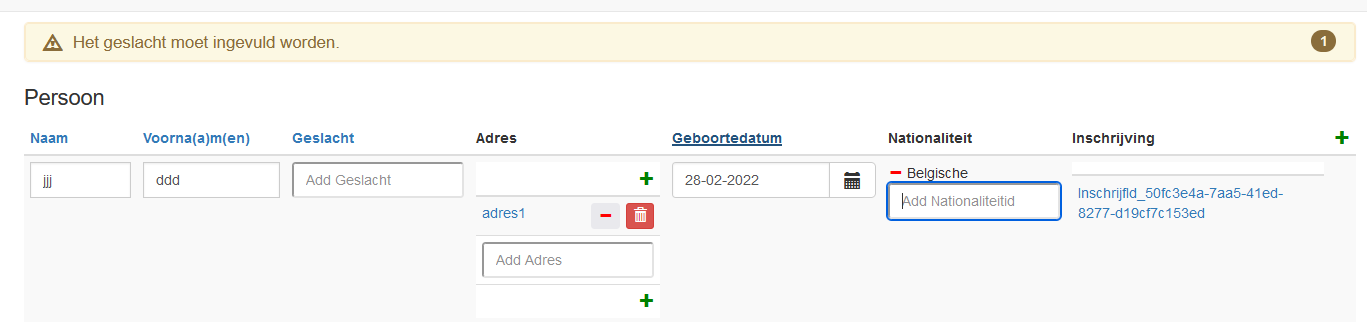
\includegraphics{docs/AF-SE/00_common/04_images/violation prototype.PNG}
    \caption{Violation \boxed{Geslacht}}
    \label{fig:violation-geslacht}
\end{figure}

\parlabel{Other}
% architecutre
% berichten nav retun messages
The use of Ampersand strongly depends on the environment in which it will be used.
The CIBG environment is quite standardized and the transition is being made to a template for registry applications.
This template is called RegisterKern.
RegisterKern includes the most common elements found in registries.
A brief exploration of RegisterKern shows that there is an overlap with some Concepts of the \acrshort{big}.
Like the Concept \boxed{Persoon}.
It appears in the \acrshort{big} and also in the RegisterKern.